\documentclass[tikz,border=4pt]{standalone}
\usepackage{xcolor}
\usetikzlibrary{arrows.meta, positioning, calc}
\definecolor{edgeblue}{HTML}{2F6FED}
\definecolor{edgegreen}{HTML}{2E8B57}
\definecolor{edgeorange}{HTML}{D9822B}
\definecolor{edgered}{HTML}{B5443C}
\definecolor{edgegray}{HTML}{F2F4F8}
\newcommand{\code}[1]{\texttt{#1}}
\begin{document}
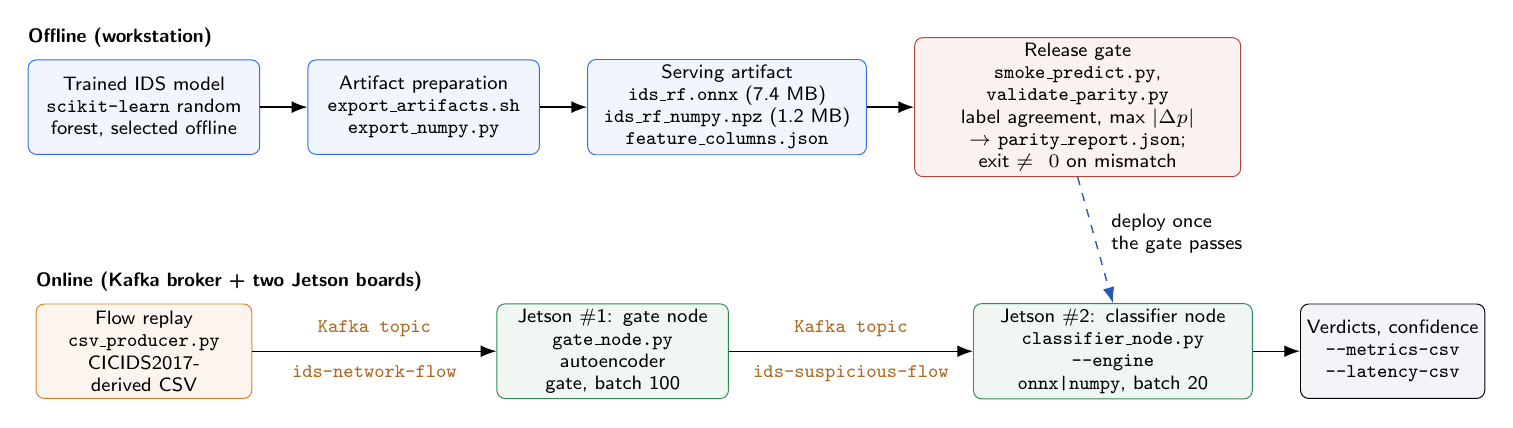
\begin{tikzpicture}[
  x=1mm, y=1mm,
  stage/.style={draw, rounded corners=3pt, align=center, minimum height=12mm,
    text width=28mm, fill=edgegray, line width=0.35pt, font=\sffamily\scriptsize, inner sep=2pt},
  blue/.style={stage, draw=edgeblue, fill=edgeblue!7},
  green/.style={stage, draw=edgegreen, fill=edgegreen!7},
  orange/.style={stage, draw=edgeorange, fill=edgeorange!8},
  red/.style={stage, draw=edgered, fill=edgered!7},
  arrow/.style={-{Latex[length=2mm]}, line width=0.5pt},
  deploy/.style={-{Latex[length=2mm]}, line width=0.5pt, dashed, color=edgeblue!80!black},
  topic/.style={font=\ttfamily\scriptsize, color=edgeorange!80!black, align=center},
  lane/.style={font=\sffamily\bfseries\scriptsize, anchor=south west, align=left, inner sep=0pt}
]
% ---------------- offline lane ----------------
\node[blue] (train) at (0, 0) {Trained IDS model\\\code{scikit-learn} random forest, selected offline};
\node[blue, right=6mm of train] (export) {Artifact preparation\\\code{export\_artifacts.sh}\\\code{export\_numpy.py}};
\node[blue, right=6mm of export, text width=34mm] (artifact)
  {Serving artifact\\\code{ids\_rf.onnx} (7.4 MB)\\\code{ids\_rf\_numpy.npz} (1.2 MB)\\\code{feature\_columns.json}};
\node[red, right=6mm of artifact, text width=40mm] (parity)
  {Release gate\\\code{smoke\_predict.py}, \code{validate\_parity.py}\\label agreement, max $|\Delta p|$ $\rightarrow$ \code{parity\_report.json}; exit $\neq 0$ on mismatch};

% ---------------- online lane ----------------
\node[orange, text width=26mm] (replay) at (0, -31) {Flow replay\\\code{csv\_producer.py}\\CICIDS2017-derived CSV};
\node[green, right=31mm of replay] (gate) {Jetson \#1: gate node\\\code{gate\_node.py}\\autoencoder gate, batch 100};
\node[green, right=31mm of gate, text width=34mm] (clf) {Jetson \#2: classifier node\\\code{classifier\_node.py}\\\code{--engine onnx|numpy}, batch 20};
\node[stage, right=6mm of clf, text width=22mm] (out) {Verdicts, confidence\\\code{--metrics-csv}\\\code{--latency-csv}};

% ---------------- arrows ----------------
\draw[arrow] (train) -- (export);
\draw[arrow] (export) -- (artifact);
\draw[arrow] (artifact) -- (parity);
\draw[arrow] (replay) -- node[topic, above=0.6mm] {Kafka topic} node[topic, below=0.6mm] {\code{ids-network-flow}} (gate);
\draw[arrow] (gate) -- node[topic, above=0.6mm] {Kafka topic} node[topic, below=0.6mm] {\code{ids-suspicious-flow}} (clf);
\draw[arrow] (clf) -- (out);
\draw[deploy] (parity.south) -- node[pos=0.45, right=1mm, font=\sffamily\scriptsize, color=black, align=left] {deploy once\\the gate passes} (clf.north);

% ---------------- lane labels ----------------
\node[lane] at ($(train.north west)+(0,1.5)$) {Offline (workstation)};
\node[lane] at ($(replay.north west)+(0,1.5)$) {Online (Kafka broker + two Jetson boards)};
\end{tikzpicture}
\end{document}
